%
\documentclass[12pt]{article}

\usepackage[usenames]{color}
\usepackage{verbatim}
\usepackage{fancyhdr}
\usepackage{graphicx}
\usepackage{amssymb,amsthm}
%\usepackage[fleqn]{amsmath}
\usepackage{amsmath}
% \usepackage[final,notref,notcite,color]{showkeys}
\usepackage[left=1in,top=1in,right=1in,bottom=1in,letterpaper]{geometry}
\renewcommand{\baselinestretch}{1.2}

\pagestyle{fancy}
\lhead{}
\chead{}
\rhead{}
\lfoot{}
\cfoot{\thepage}
\rfoot{}



%% editing
\usepackage[shortlabels]{enumitem}
\usepackage[normalem]{ulem}

%% macros for commenting
\usepackage{changepage}
\usepackage{mathtools}
\usepackage[normalem]{ulem} % to use \sout

%% math packages
% \usepackage{amsmath} % not needed for Springer
\usepackage{amssymb}
\usepackage{mathrsfs}

%\usepackage{subfigure}
%\usepackage{url}

%% a light-weight algorithm environment
\newtheorem{algo}{Algorithm}

%% highlighting and commenting
\newcommand{\outline}[1]{{\color{brown}#1}}
\newcommand{\rev}[1]{{\color{blue}#1}}
\newcommand{\remove}[1]{{\sout{#1}}}
\newcommand{\cut}[1]{{}}

%% macros for letters

\newcommand{\va}{{\mathbf{a}}}
\newcommand{\vb}{{\mathbf{b}}}
\newcommand{\vc}{{\mathbf{c}}}
\newcommand{\vd}{{\mathbf{d}}}
\newcommand{\ve}{{\mathbf{e}}}
\newcommand{\vf}{{\mathbf{f}}}
\newcommand{\vg}{{\mathbf{g}}}
\newcommand{\vh}{{\mathbf{h}}}
\newcommand{\vi}{{\mathbf{i}}}
\newcommand{\vj}{{\mathbf{j}}}
\newcommand{\vk}{{\mathbf{k}}}
\newcommand{\vl}{{\mathbf{l}}}
\newcommand{\vm}{{\mathbf{m}}}
\newcommand{\vn}{{\mathbf{n}}}
\newcommand{\vo}{{\mathbf{o}}}
\newcommand{\vp}{{\mathbf{p}}}
\newcommand{\vq}{{\mathbf{q}}}
\newcommand{\vr}{{\mathbf{r}}}
\newcommand{\vs}{{\mathbf{s}}}
\newcommand{\vt}{{\mathbf{t}}}
\newcommand{\vu}{{\mathbf{u}}}
\newcommand{\vv}{{\mathbf{v}}}
\newcommand{\vw}{{\mathbf{w}}}
\newcommand{\vx}{{\mathbf{x}}}
\newcommand{\vy}{{\mathbf{y}}}
\newcommand{\vz}{{\mathbf{z}}}

\newcommand{\ta}{{\tilde{a}}}
\newcommand{\tb}{{\tilde{b}}}
\newcommand{\tc}{{\tilde{c}}}
\newcommand{\td}{{\tilde{d}}}
\newcommand{\te}{{\tilde{e}}}
\newcommand{\tf}{{\tilde{f}}}
\newcommand{\tg}{{\tilde{g}}}

\newcommand{\ti}{{\tilde{i}}}
\newcommand{\tj}{{\tilde{j}}}
\newcommand{\tk}{{\tilde{k}}}
\newcommand{\tl}{{\tilde{l}}}
\newcommand{\tm}{{\tilde{m}}}
\newcommand{\tn}{{\tilde{n}}}

\newcommand{\tp}{{\tilde{p}}}
\newcommand{\tq}{{\tilde{q}}}

\newcommand{\ts}{{\tilde{s}}}

\newcommand{\tu}{{\tilde{u}}}
\newcommand{\tv}{{\tilde{v}}}
\newcommand{\tw}{{\tilde{w}}}
\newcommand{\tx}{{\tilde{x}}}
\newcommand{\ty}{{\tilde{y}}}
\newcommand{\tz}{{\tilde{z}}}

\newcommand{\vA}{{\mathbf{A}}}
\newcommand{\vB}{{\mathbf{B}}}
\newcommand{\vC}{{\mathbf{C}}}
\newcommand{\vD}{{\mathbf{D}}}
\newcommand{\vE}{{\mathbf{E}}}
\newcommand{\vF}{{\mathbf{F}}}
\newcommand{\vG}{{\mathbf{G}}}
\newcommand{\vH}{{\mathbf{H}}}
\newcommand{\vI}{{\mathbf{I}}}
\newcommand{\vJ}{{\mathbf{J}}}
\newcommand{\vK}{{\mathbf{K}}}
\newcommand{\vL}{{\mathbf{L}}}
\newcommand{\vM}{{\mathbf{M}}}
\newcommand{\vN}{{\mathbf{N}}}
\newcommand{\vO}{{\mathbf{O}}}
\newcommand{\vP}{{\mathbf{P}}}
\newcommand{\vQ}{{\mathbf{Q}}}
\newcommand{\vR}{{\mathbf{R}}}
\newcommand{\vS}{{\mathbf{S}}}
\newcommand{\vT}{{\mathbf{T}}}
\newcommand{\vU}{{\mathbf{U}}}
\newcommand{\vV}{{\mathbf{V}}}
\newcommand{\vW}{{\mathbf{W}}}
\newcommand{\vX}{{\mathbf{X}}}
\newcommand{\vY}{{\mathbf{Y}}}
\newcommand{\vZ}{{\mathbf{Z}}}

\newcommand{\cA}{{\mathcal{A}}}
\newcommand{\cB}{{\mathcal{B}}}
\newcommand{\cC}{{\mathcal{C}}}
\newcommand{\cD}{{\mathcal{D}}}
\newcommand{\cE}{{\mathcal{E}}}
\newcommand{\cF}{{\mathcal{F}}}
\newcommand{\cG}{{\mathcal{G}}}
\newcommand{\cH}{{\mathcal{H}}}
\newcommand{\cI}{{\mathcal{I}}}
\newcommand{\cJ}{{\mathcal{J}}}
\newcommand{\cK}{{\mathcal{K}}}
\newcommand{\cL}{{\mathcal{L}}}
\newcommand{\cM}{{\mathcal{M}}}
\newcommand{\cN}{{\mathcal{N}}}
\newcommand{\cO}{{\mathcal{O}}}
\newcommand{\cP}{{\mathcal{P}}}
\newcommand{\cQ}{{\mathcal{Q}}}
\newcommand{\cR}{{\mathcal{R}}}
\newcommand{\cS}{{\mathcal{S}}}
\newcommand{\cT}{{\mathcal{T}}}
\newcommand{\cU}{{\mathcal{U}}}
\newcommand{\cV}{{\mathcal{V}}}
\newcommand{\cW}{{\mathcal{W}}}
\newcommand{\cX}{{\mathcal{X}}}
\newcommand{\cY}{{\mathcal{Y}}}
\newcommand{\cZ}{{\mathcal{Z}}}

\newcommand{\ri}{{\mathrm{i}}}
\newcommand{\rr}{{\mathrm{r}}}

\newcommand{\EE}{{\mathbb{E}}}


%% macros for math notions and operators

\newcommand{\RR}{\mathbb{R}}
\newcommand{\CC}{\mathbb{C}}
\newcommand{\ZZ}{\mathbb{Z}}
\renewcommand{\SS}{{\mathbb{S}}}
\newcommand{\SSp}{\mathbb{S}_{+}}
\newcommand{\SSpp}{\mathbb{S}_{++}}
\newcommand{\sign}{\mathrm{sign}}
\newcommand{\vzero}{\mathbf{0}}
\newcommand{\vone}{{\mathbf{1}}}

\newcommand{\st}{{\text{s.t.}}} % subject to
\newcommand{\St}{{\mathrm{subject~to}}} % subject to
\newcommand{\op}{{\mathrm{op}}} % subscript for operator norm
\newcommand{\opt}{{\mathrm{opt}}} % subscript for optimal solution
%\newcommand{\supp}{{\mathrm{supp}}} % support
\newcommand{\Prob}{{\mathrm{Prob}}} % probability
\newcommand{\Diag}{{\mathrm{Diag}}} % vector -> diagonal matrix
%\newcommand{\diag}{{\mathrm{diag}}} % matrix diagonal -> vector
\newcommand{\dom}{{\mathrm{dom}}} % domain
\newcommand{\range}{{\mathrm{range}}} % domain
%\newcommand{\grad}{{\nabla}}    % gradient
\newcommand{\tr}{{\mathrm{tr}}} % trace
\newcommand{\TV}{{\mathrm{TV}}} % total variation
\newcommand{\Proj}{{\mathrm{Proj}}}
\newcommand{\prj}{{\mathrm{prj}}}
\newcommand{\prox}{\mathbf{prox}}
\newcommand{\refl}{\mathbf{refl}}
\newcommand{\reflh}{\refl^{\bH}}
\newcommand{\proxh}{\prox^{\bH}}
\newcommand{\minimize}{\text{minimize}}
\newcommand{\bgamma}{\boldsymbol{\gamma}}
\newcommand{\bsigma}{\boldsymbol{\sigma}}
\newcommand{\bomega}{\boldsymbol{\omega}}
\newcommand{\blambda}{\boldsymbol{\lambda}}
\newcommand{\bH}{\vH}
\newcommand{\bbH}{\mathbb{H}}
\newcommand{\bB}{\boldsymbol{\cB}}
\newcommand{\Tau}{\mathrm{T}}
\newcommand{\tnabla}{\widetilde{\nabla}}
\newcommand{\TDRS}{T_{\mathrm{DRS}}}
\newcommand{\TPRS}{T_{\mathrm{PRS}}}
\newcommand{\TFBS}{T_{\mathrm{FBS}}}
\newcommand{\best}{\mathrm{best}}
\newcommand{\kbest}{k_{\best}}
\newcommand{\diff}{\mathrm{diff}}
\newcommand{\barx}{\bar{x}}
\newcommand{\xgbar}{\bar{x}_g}
\newcommand{\xfbar}{\bar{x}_f}
\newcommand{\hatxi}{\hat{\xi}}
\newcommand{\xg}{x_g}
\newcommand{\xf}{x_f}
\newcommand{\du}{\mathrm{d}u}
\newcommand{\dy}{\mathrm{d}y}
\newcommand{\kconvergence}{\stackrel{k \rightarrow \infty}{\rightarrow }}
\DeclareMathOperator{\shrink}{shrink} % shrinkage
\DeclareMathOperator*{\argmin}{arg\,min}
\DeclareMathOperator*{\argmax}{arg\,max}
\DeclareMathOperator*{\Min}{minimize}
\DeclareMathOperator*{\Max}{maximize}
\DeclareMathOperator*{\Fix}{Fix}
\DeclareMathOperator*{\zer}{zer}
\DeclareMathOperator*{\nablah}{\nabla^{\bH}}
\DeclareMathOperator*{\gra}{gra}
\DeclarePairedDelimiter{\dotpb}{\langle}{\rangle_{\bH}}
\DeclarePairedDelimiter{\dotpv}{\langle}{\rangle_{\vH}}
\DeclarePairedDelimiter{\dotp}{\langle}{\rangle}

%% macros for environments math equations

\newcommand{\MyFigure}[1]{../fig/#1}

\newcommand{\bc}{\begin{center}}
\newcommand{\ec}{\end{center}}

\newcommand{\bdm}{\begin{displaymath}}
\newcommand{\edm}{\end{displaymath}}

\newcommand{\beq}{\begin{equation}}
\newcommand{\eeq}{\end{equation}}

\newcommand{\bfl}{\begin{flushleft}}
\newcommand{\efl}{\end{flushleft}}

\newcommand{\bt}{\begin{tabbing}}
\newcommand{\et}{\end{tabbing}}

\newcommand{\beqn}{\begin{align}}
\newcommand{\eeqn}{\end{align}}

\newcommand{\beqs}{\begin{align*}} % no equation numbers
\newcommand{\eeqs}{\end{align*}}  % no equation numbers

%% macros for theorem-like environments

%\newtheorem{theorem}{Theorem}
\newtheorem{assumption}{Assumption}
%\newtheorem{condition}{Condition}
%\newtheorem{rul}{Rule}
%\newtheorem{definition}{Definition}
%\newtheorem{corollary}{Corollary}
%\newtheorem{remark}{Remark}
%\newtheorem{lemma}{Lemma}
%\newtheorem{proposition}{Proposition}
%\newtheorem{example}{Example}
%\newtheorem{proof}{Proof}

%%%%%%%%%%%%%%%%%%%%%%%%%%%%%%%%%%%%%%%%%%%%%

\title{Assignment 4 of MATP4820}
\author{Izaak King}
\date{February 23, 2026}



\begin{document}

\maketitle

\section*{Problem 1}
Consider the unconstrained quadratic minimization problem:
\begin{equation}\label{eq:quad-min}\tag{QuadMin}
\Min_\vx f(\vx) = \frac{1}{2}\vx^\top \vA \vx - \vb^\top \vx
\end{equation}
where $\vA\in\RR^{n\times n}$ is a symmetric positive definite matrix, and $\vb\in\RR^n$. 
\begin{enumerate}
\item Let $\vA=\left[\begin{array}{cc}4 & -2\\ -2 & 3\end{array}\right]$ and $\vb=\left[\begin{array}{r}2 \\ 1\end{array}\right]$. Set the initial vector $\vx^0=\left[\begin{array}{r}0 \\ 0\end{array}\right]$. Do by hand the conjugate gradient method to find the \textbf{exact solution}. 

\vspace{8mm}

First, take $x^{(1)} = 
\begin{bmatrix}
0 \\
0
\end{bmatrix}$

Iteration 0:

\[ r^{(1)} = Ax^{(1)} - b = -b =
\begin{bmatrix}
-2 \\
-1
\end{bmatrix}\]

\[ p^{(1)} = -r^{(1)} = \begin{bmatrix}
2 \\
1
\end{bmatrix}
\]

Iteration 1: k = 1

\[Ap^{(1)} = \begin{bmatrix}
4 & -2\\
-2 & 3
\end{bmatrix}\begin{bmatrix}
2 \\
1
\end{bmatrix} = \begin{bmatrix}
6 \\
-1
\end{bmatrix} \]

\[ \alpha^{(1)} = - \frac{\langle p^{(k)}, r^{(k)} \rangle}{\langle p^{(1)}, Ap^{(1)}\rangle} = - \frac{\langle \begin{bmatrix}
-2 \\
-1
\end{bmatrix},\begin{bmatrix}
2 \\
1
\end{bmatrix}\rangle}{\langle \begin{bmatrix}
2 \\
1
\end{bmatrix}, \begin{bmatrix}
6 \\
-1
\end{bmatrix} \rangle} = - \left(-\frac{5}{11}\right) = \frac{5}{11}\]

\[x^{(2)} = x^{(1)} + \alpha^{(1)}p^{(1)} = \begin{bmatrix}
0 \\
0
\end{bmatrix} + \frac{5}{11} \begin{bmatrix}
2 \\
1
\end{bmatrix} =\begin{bmatrix}
\frac{10}{11} \\
\frac{5}{11}
\end{bmatrix}\]

\[ r^{(2)} = Ax^{(2)} - b = \begin{bmatrix}
4 & -2 \\
-2 & 3
\end{bmatrix}\begin{bmatrix}
\frac{10}{11} \\
\frac{5}{11}
\end{bmatrix} - \begin{bmatrix}
2 \\
1
\end{bmatrix} = \begin{bmatrix}
\frac{30}{11} \\
-\frac{5}{11}
\end{bmatrix} - \begin{bmatrix}
2 \\
1
\end{bmatrix} = \begin{bmatrix}
\frac{8}{11} \\
-\frac{16}{11}
\end{bmatrix}\]

\[ \beta^{(2)} = \frac{\langle r^{(2)}, Ap^{(1)} \rangle}{\langle p^{(1)}, Ap^{(1)}\rangle} = \frac{\langle \begin{bmatrix}
\frac{8}{11} \\
-\frac{16}{11}
\end{bmatrix}, \begin{bmatrix}
6 \\
-1
\end{bmatrix}\rangle}{\langle \begin{bmatrix}
2 \\
1
\end{bmatrix}, \begin{bmatrix}
6 \\
-1
\end{bmatrix}\rangle} = \frac{\frac{64}{11}}{11} = \frac{64}{121}\]

\[p^{(2)} = -r^{(2)} + \beta^{(2)}p^{(1)} = -\begin{bmatrix}
\frac{8}{11} \\
-\frac{16}{11}
\end{bmatrix} + \frac{64}{121} \begin{bmatrix}
2 \\
1
\end{bmatrix} = \begin{bmatrix}
\frac{40}{121} \\
\frac{240}{121}
\end{bmatrix}\]

Iteration 2: k = 2

\[ Ap^{(2)} = \begin{bmatrix}
4 & -2 \\
-2 & 3
\end{bmatrix}
\begin{bmatrix}
\frac{40}{121} \\
\frac{240}{121}
\end{bmatrix} = \begin{bmatrix}
-\frac{320}{121} \\
\frac{640}{121}
\end{bmatrix}\]

\[\alpha^{(2)} = - \frac{\langle p^{(2)} , r^{(2)} \rangle}{\langle p^{(2)}, Ap^{(2)}\rangle} = \frac{\langle \begin{bmatrix}
\frac{40}{121} \\
\frac{240}{121}
\end{bmatrix}, \begin{bmatrix}
\frac{8}{11} \\
\frac{-16}{11}
\end{bmatrix} \rangle}{\langle \begin{bmatrix}
\frac{40}{121} \\
\frac{240}{121}
\end{bmatrix}, \begin{bmatrix}
-\frac{320}{121} \\
\frac{640}{121}
\end{bmatrix}} = - \frac{-\frac{3520}{1331}}{\frac{140800}{14641}} = \frac{11}{40} \]

\[x^{(3)} = x^{(2)} + \alpha^{(2)}p^{(2)} = \begin{bmatrix}
\frac{10}{11} \\
\frac{5}{11}
\end{bmatrix} + \frac{11}{40} \begin{bmatrix}
\frac{40}{121} \\
\frac{240}{121}
\end{bmatrix} = \begin{bmatrix}
1 \\
1
\end{bmatrix}\]

\[ r^{(3)} = Ax^{(3)} - b = \begin{bmatrix}
4 & -2 \\
-2 & 3
\end{bmatrix}\begin{bmatrix}
1 \\
1
\end{bmatrix} - \begin{bmatrix}
2 \\
1
\end{bmatrix} = \begin{bmatrix}
0 \\
0
\end{bmatrix}\]

Thus, we have $r^{(3)} = \begin{bmatrix}
0 \\
0
\end{bmatrix}$, so we have found the exact solution and we stop iterating. We get the exact solution of $x^{(3)} = \begin{bmatrix}
1 \\
1
\end{bmatrix}$


\newpage

\item Use the instructor's provided file \verb|quadMin_cg.m| to write a Matlab function \verb|quadMin_cg| with input $\vA$, $\vb$, initial vector $\vx0$, and tolerance \verb|tol|, and with stopping condition $\|\nabla f(\vx^k)\| \le \text{tol}$. Also test your function by running the provided test file \verb|test_cg.m| and compare to the instructor's function. Print your code and the results you get. Make discussions on what you observe for the difference between your steepest gradient method solver (from the 3rd assignment) and your conjugate gradient method solver.
\end{enumerate}

\vspace{8mm}

\noindent \textbf{Conjugate Gradient Method (quadMin\_cg.m) Solver}
\vspace{4mm}
\begin{verbatim}
function [x, hist_res] = quadMin_cg(A,b,x0,tol)

% conjugate gradient method for solving
% min_x 0.5*x'*A*x - b'*x

% get the size of the problem
n = length(b);

x = x0;

% compute vector r, i.e., gradient of the objective
r = A * x - b;

% set the first p vector as negative gradient
p = -r;

% evaluate the norm of gradient
res = norm(r);

% save the value of res
hist_res = res;

while res > tol
    
    % compute A * p once

    Apk = A * p;

    % compute <p, Apk> once
    
    pDotApk = dot(p, Apk);

    % compute alpha
    
    alpha = - dot(p, r) / pDotApk;
    
    % update x 
    
    x = x + alpha * p;
    
    % update r
    
    r = A * x - b;
    
    % compute beta
    
    beta = dot(r, Apk) / pDotApk;
    
    % obtain the new p vector
    
    p = -r + beta * p;
    
    % evaluate the norm of residual vector r
    res = norm(r);
    
    % save the value of res
    hist_res = [hist_res; res];
end

end

\end{verbatim}

\newpage

\noindent \textbf{test\_cg.m Output}


\begin{verbatim}
>> test_cg
Results by student code
Total running time is 0.0020
Final objective value is -4551.8686
Results by Instructor code
Total running time is 0.0014
Final objective value is -4551.8686
Results by Student GD code
Total running time is 0.0269
Final objective value is -4551.8686
Results by Instructor GD code
Total running time is 0.0281
Final objective value is -4551.8686
\end{verbatim}

\vspace{4mm}

\noindent \textbf{NOTE: For comparisons, we will use the performance of both algorithms I created, rather than the instructor's}

\vspace{4mm}

\noindent \textbf{CG Method Plot}

\begin{figure}[h!] % [h!] suggests placing the figure "here" if possible
    \centering % Centers the image and caption
    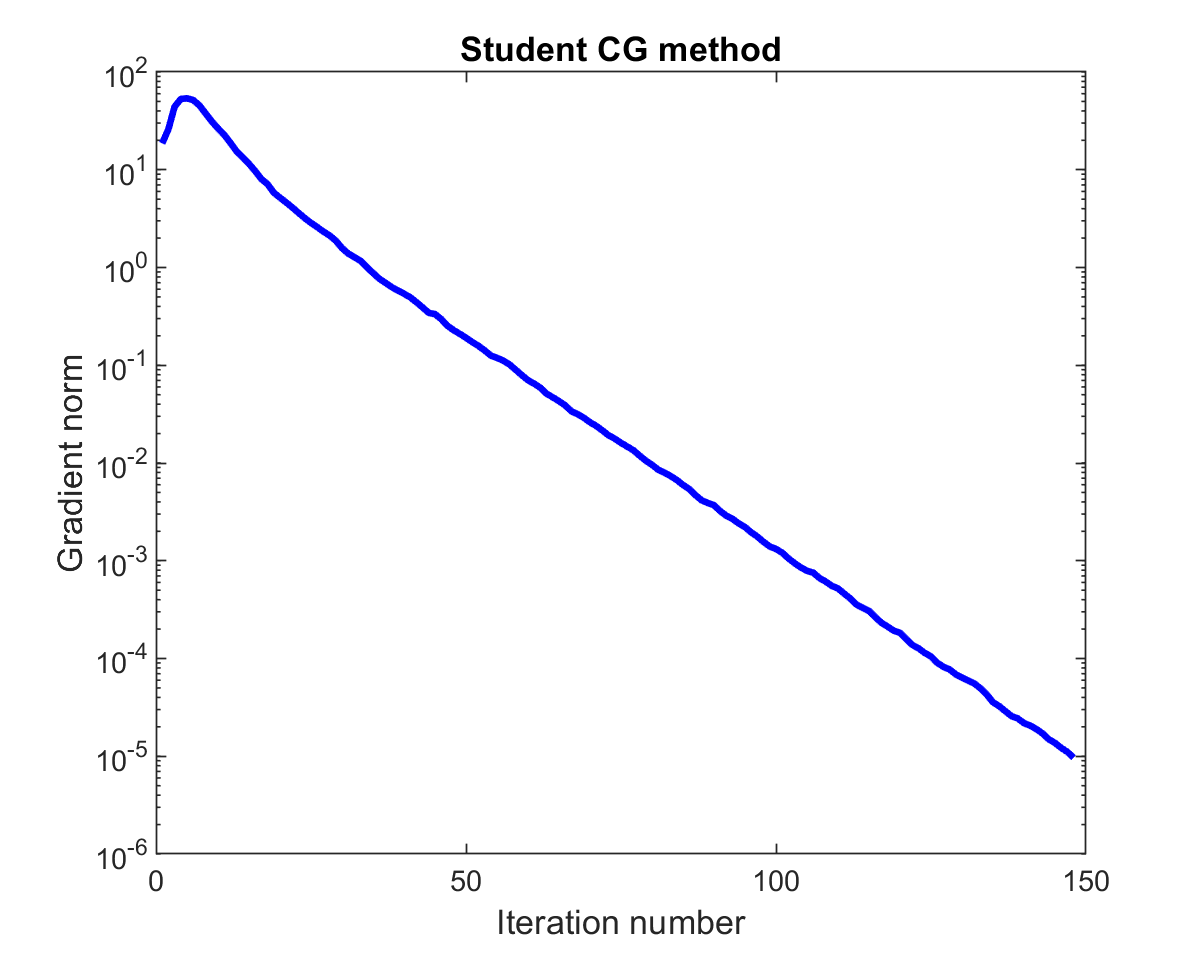
\includegraphics[width=0.7\linewidth]{student_cg.png}
    \caption{Plot outputted by running Conjugate Gradient method.} % Adds a caption
    \label{fig:my_image} % Adds a label for cross-referencing
\end{figure}

\newpage

\noindent \textbf{GD Method Plot}

\begin{figure}[h!] % [h!] suggests placing the figure "here" if possible
    \centering % Centers the image and caption
    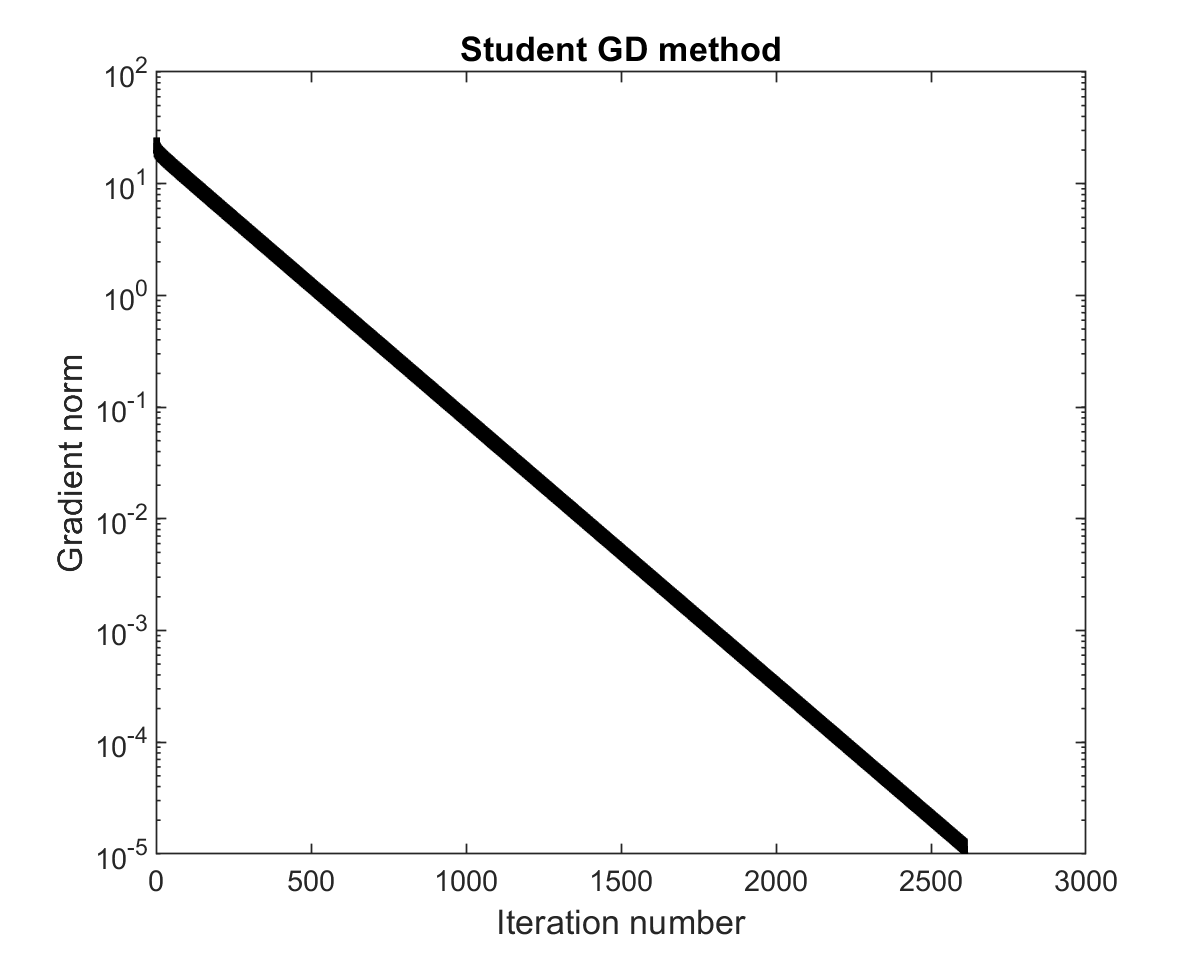
\includegraphics[width=0.7\linewidth]{student_gd.png}
    \caption{Plot outputted by running Gradient Descent method.} % Adds a caption
    \label{fig:my_image} % Adds a label for cross-referencing
\end{figure}

\noindent Based on the outputs from our testing, as well as the plots of total iterations, it is clear the Conjugate Gradient method performs much better than the Gradient Descent Method with this test. The running time is much faster, with Conjugate Gradient taking 0.0020 and Gradient Descent taking 0.0281. Similarly, Conjugate Gradient takes about 150 iterations while Gradient Descent takes over 2500, showcasing Conjugate Gradient's significant improvement.

\newpage


\section*{Problem 2}
For ill-conditioned problems, the conjugate gradient (CG) method may converge very slowly, and a better method is the preconditioned conjugate gradient (PCG) method. Consider the quadratic minimization problem in \eqref{eq:quad-min} stated in Problem 1.
Write a solver for \eqref{eq:quad-min} by the PCG method. We will use a non-singular triangular matrix $\vC$ as the preconditioner.

\begin{enumerate}
\item Let $\vC\in \RR^{n\times n}$ be a non-singular upper triangular matrix. Write a solver \verb|pcg_linsolv| for the linear system $\vC^\top \vC \vy = \vr$. Treat $\vC$ and $\vr$ as the input of the solver. Recall that to solve the linear system, we can first solve $\vC^\top\vz = \vr$ by forward substitution and then solve $\vC\vy = \vz$ by back substitution. [\textbf{Note}: you will need to use for-loop in your solver. You CANNOT use MATLAB's solver to directly solve the linear system.]

\vspace{8mm}

\noindent \textbf{pcg\_linsolv Function}
\vspace{4mm}
\begin{verbatim}
function [y] = pcg_linsolv(C, r)

    % Initialize C^T, solution vectors z and y, and matrix size n
    CT = transpose(C);
    n = size(CT, 1);
    z = zeros(n, 1);
    y = zeros(n, 1);

    % Forward substitution
    for i = 1:n

        % Add known values up until diagonal
        summation = 0;
        for j = 1:i-1
            summation = summation + CT(i, j) * z(j);
        end

        % Get current diagonal value
        z(i) = (r(i) - summation) / CT(i, i);
    end

    % Backward substitution
    for i = n:-1:1

        % Add known values up until diagonal
        summation = 0;
        for j = i + 1:n
            summation = summation + C(i, j) * y(j);
        end

        % Get current diagonal value
        y(i) = (z(i) - summation) / C(i, i);
    end
end
\end{verbatim}

\newpage

\item Write a Matlab function \verb|quadMin_pcg| with input $\vA$, $\vC$, and $\vb$, where $\vC$ is a non-singular upper triangular matrix, used as the conditioning matrix. Within your PCG solver, use \verb|pcg_linsolv| that you develop in the previous question as the linear solver for solving linear systems in the form of $\vC^\top \vC \vy = \vr$. Also test your function by running the provided test file \verb|test_pcg.m| and compare to the instructor's function. Print your code and the results you get. [\textbf{Hint}: to debug your PCG solver, you can use MATLAB's linear system solver to directly solve $\vC^\top \vC \vy = \vr$. But your final version of your PCG solver MUST use \verb|pcg_linsolv| that you develop.]

\end{enumerate}

\vspace{8mm}

\noindent \textbf{Preconditioned Conjugate Gradient (quadMin\_pcg) Function}
\vspace{4mm}
\begin{verbatim}
function [x, hist_res] = quadMin_pcg(A,C,b,x0,tol)

% conjugate gradient method for solving
% min_x 0.5*x'*A*x - b'*x

% get the size of the problem
n = length(b);

x = x0;

% compute vector r, i.e., gradient of the objective
r = A * x - b;

% compute first y
y = pcg_linsolv(C, r);

% set the first p vector 
p = -y;

% evaluate the norm of gradient
res = norm(r);

% save the value of res
hist_res = res;

while res > tol

    % compute rk dot yk once

    rDoty = dot(r, y);

    % compute A * p once

    Ap = A*p;

    % compute alpha
    
    alpha = rDoty / dot(p, Ap);
    
    % update x 
    
    x = x + alpha*p;
    
    % update r
    
    r = r + alpha * Ap;

    % compute updated y once

    yNext = pcg_linsolv(C, r);
    
    % compute beta
    
    beta = dot(r, yNext) / rDoty;
    
    % obtain the new p vector
    
    p = -yNext + beta * p;

    % update y

    y = yNext;
    
    % evaluate the norm of residual vector r
    res = norm(r);
    
    % save the value of res
    hist_res = [hist_res; res];
end

end

\end{verbatim}

\noindent \textbf{test\_pcg.m Output}
\begin{verbatim}
>> test_pcg
Student solver: Total iteration is 130
Total running time is 2.8527
Final objective value is -1.4159
Instructor pcg solver: Total iteration is 130
Total running time is 0.7172
Final objective value is -1.4159
Instructor cg solver: Total iteration is 287
Final objective value is -1.4159
\end{verbatim}

\vspace{4mm}

\noindent Thus we see the Preconditioned Conjugate Gradient Method arrives at the final objective value in less than half the iterations as the instructor's Conjugate Gradient solver. Our PCG method takes 130 total iterations, while the CG method takes 287 iterations to arrive at the same final objective value.

\newpage

\section*{Problem 3}
 Let $f(x) = x^2 + e^{-x} +2\cos x, x\in\RR$. 

\begin{enumerate}
\item Prove that this function is convex and show by graph that this function has a minimizer. 

\vspace{8mm}

\begin{proof}First, to prove$f(x)$ is convex, we will show $f''(x) \geq 0$ for any $x \in \mathbb{R}$ 
\begin{adjustwidth}{2em}{} Now with 

\[f(x) = x^2 + e^{-x} + 2\cos x \]

\[f'(x) = 2x - e^{-x} - 2\sin x \]

\[f''(x) = 2 + e^{-x} - 2\cos x \]

Thus, we must show

\[f''(x) = 2 + e^{-x} - 2\cos x \geq 0 \text{ for all } x \in \mathbb{R}\]

First note, 

\[ -1 \leq \cos x \leq 1 \implies -2 \leq 2\cos x \leq 2\]

Then,

\[ 2 + e^{-x} - 2 \leq 2 + e^{-x} - 2 \cos x \leq 2 + e^{-x} + 2 \implies e^{-x} \leq 2 + e^{-x} - 2\cos x\]

Now, $e^{-x} > 0$ for all $x \in \mathbb{R}$. Thus,

\[f''(x) = 2 + e^{-x} - 2\cos x \geq e^{-x} > 0 \text{ for all } x \in \mathbb{R}\]

Therefore, $f''(x) \geq 0$ for all $x \in \mathbb{R}$, and $f(x)$ is convex.

\end{adjustwidth}

\end{proof}

\newpage

\noindent Now, showing by graph $f(x)$ has a minimum
\vspace{8mm}

\noindent \textbf{Hand-Drawn Graph}

\begin{figure}[h!] % [h!] suggests placing the figure "here" if possible
    \centering % Centers the image and caption
    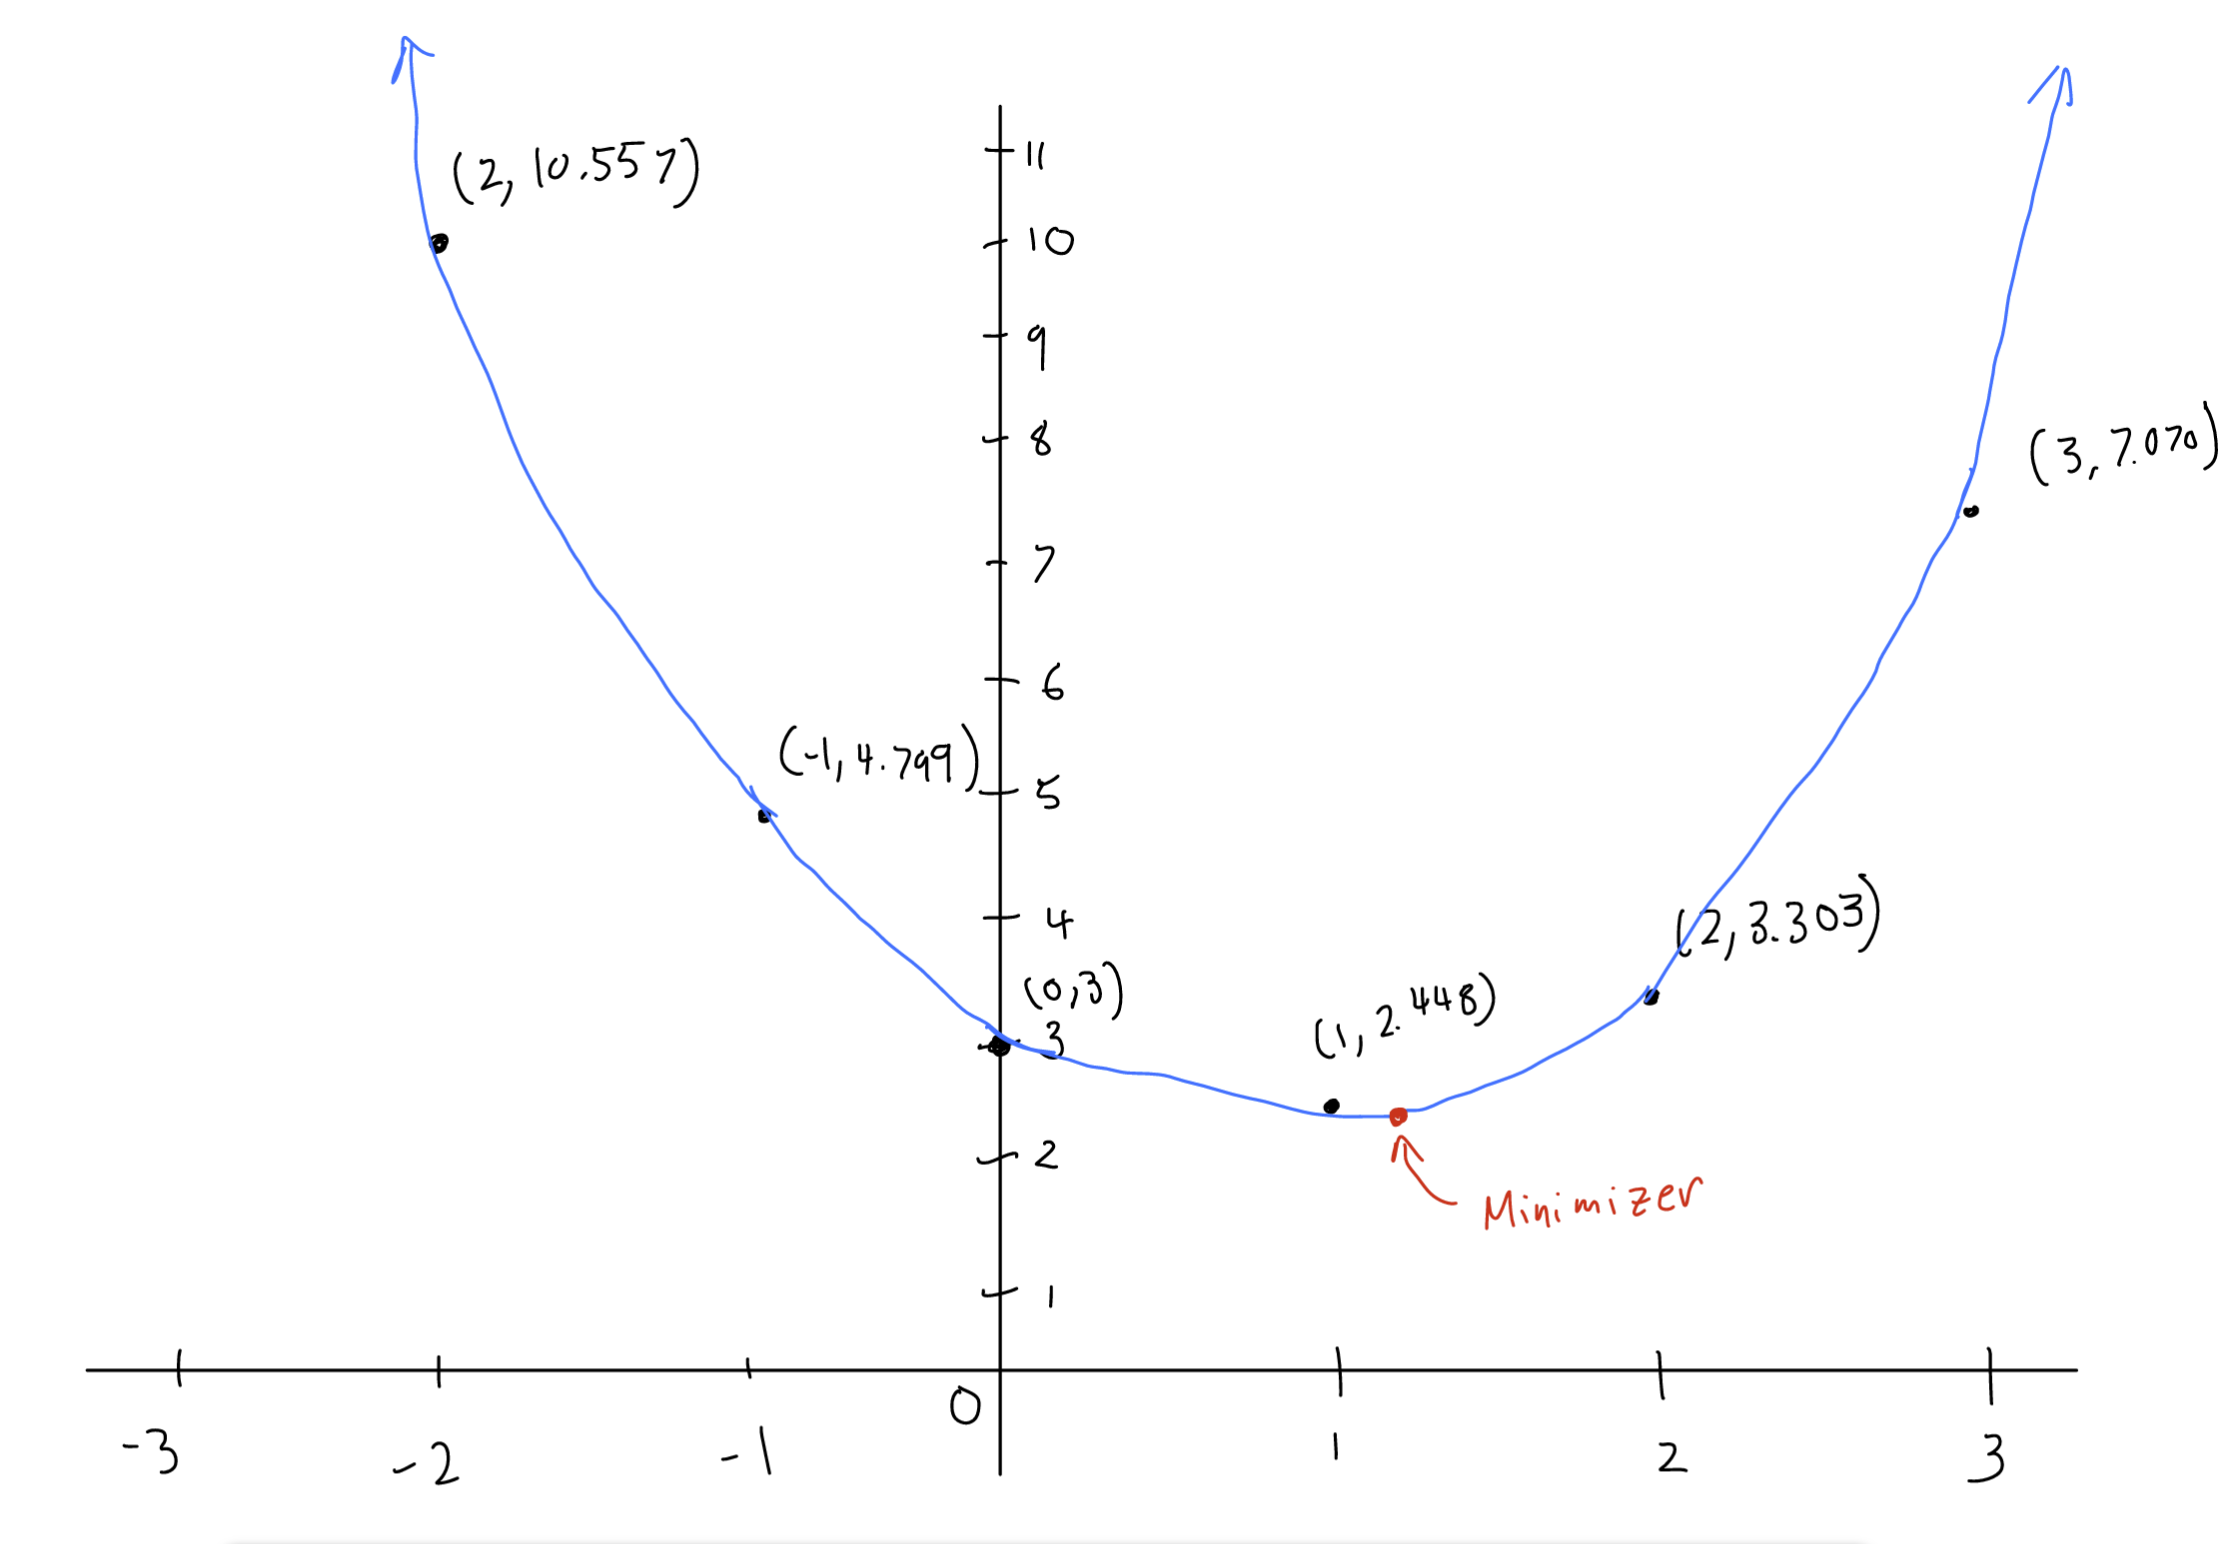
\includegraphics[width=0.7\linewidth]{handdrawn graph.png}
    \caption{Hand-drawn graph of $f(x)$.} % Adds a caption
    \label{fig:my_image} % Adds a label for cross-referencing
\end{figure}

\noindent \textbf{Computed Graph}

\begin{figure}[h!] % [h!] suggests placing the figure "here" if possible
    \centering % Centers the image and caption
    \includegraphics[width=0.7\linewidth]{Desmos graph.png}
    \caption{Computed graph of $f(x)$.} % Adds a caption
    \label{fig:my_image} % Adds a label for cross-referencing
\end{figure}

\noindent Thus in both graphs, hand-drawn and computed, we see $f(x)$ has a clear minimizer value occurring just past $x = 1$. Since the graph continues to strictly increase in both directions to the left and right of this minimizer, we see this a global minimum of $f(x)$. 

\newpage 

\item Start from $x^{(0)}=2$ and do 3 iterations of the Newton's method to find an approximate minimizer of $f(x)$ by hand (calculator is allowed).


\end{enumerate}

First, we have 

\[f(x) = x^2 + e^{-x} + 2\cos x \]

\[f'(x) = 2x - e^{-x} - 2\sin x \]

\[f''(x) = 2 + e^{-x} - 2\cos x \]

We will use Newton's iteration:

\[x^{(k + 1)} = x^{(k)} - \frac{f'(x^{(k)})}{f''(x^{(k)})}\]

Iteration 1:

\[x^{(1)} = x^{(0)} - \frac{f'(x^{(0)})}{f''(x^{(0)})} = 2 - \frac{(2(2) - e^{-2} - 2 \sin (2))}{2 + e^{-2} - 2\cos (2)} \approx 1.3105 \]

Iteration 2:

\[x^{(2)} = x^{(1)} - \frac{f'(x^{(1)})}{f''(x^{(1)})} \approx 1.3105 - \frac{(2(1.3105) - e^{-1.3105} - 2 \sin (1.3105)}{2 + e^{-1.3105} - 2\cos (1.3105)} \approx 1.0719\]

Iteration 3:

\[x^{(3)} = x^{(2)} - \frac{f'(x^{(2)})}{f''(x^{(2)})} \approx 1.0719 - \frac{(2(1.0719) - e^{-1.0719} - 2 \sin (1.0719)}{2 + e^{-1.0719} - 2\cos (1.0719)} \approx 1.0393\] 

Thus after 3 iterations, we get the approximate minimizer $x^{(3)} \approx 1.0393$


\end{document}
